\section{Gaussian Mixture Models}

\medskip

Some key R commands are:
\begin{itemize}
    \item \texttt{library(mclust)}: Loads the \texttt{mclust} package for Gaussian mixture modeling and model-based clustering.
    
    \item \texttt{gmm <- Mclust(data)}: Fits a Gaussian mixture model to \texttt{data}, selecting the number of components and covariance structure using BIC.
    
    \item \texttt{gmm\$loglik}: Returns the maximized log-likelihood of the fitted model.
    
    \item \texttt{gmm\$parameters\$pro}: Returns the estimated mixing proportions of the components.
    
    \item \texttt{gmm\$parameters\$mean}: Returns the estimated component means.
    
    \item \texttt{gmm\$parameters\$variance}: Returns the estimated covariance matrices and variance structure information.
\end{itemize}

\medskip

A \emph{Gaussian Mixture Model} (GMM) approaches clustering from a probabilistic perspective. Rather than partitioning the data directly, we assume that the observed points were generated by several underlying
multivariate normal distributions, combined together in certain proportions.

The GMM framework assumes that each observation was generated from one of $K$ multivariate Gaussian distributions. Each Gaussian represents a
cluster, characterized by its own mean vector and covariance matrix. The overall population distribution is therefore a \emph{mixture} of these Gaussian components.

Conceptually, the data-generating process can be described in two steps. First, a component (or cluster) is selected according to some set of mixing proportions. Second, a data point is drawn from the multivariate
normal distribution associated with that component. The observed data are the result of repeating this process many times.

This viewpoint contrasts sharply with methods such as $K$-means. In $K$-means, each point is deterministically assigned to exactly one cluster, producing a hard partition of the data. In a GMM, by contrast,
cluster membership is \emph{probabilistic}. For each observation $x_i$, the model produces a collection of probabilities indicating how likely it is that $x_i$ originated from each of the $K$ Gaussian components.

These probabilities allow GMMs to represent uncertainty in cluster membership. In regions where clusters overlap, a point may have substantial probability of belonging to multiple components. This makes the model more flexible than purely geometric partitioning methods and better suited to data whose structure cannot be captured by spherical or well-separated clusters.

\bigskip

\subsection*{Theoretical Foundations}

\medskip

A Gaussian Mixture Model is parameterized by three types of quantities. Each component $k$ has:

\begin{itemize}
    \item A mean vector $\mu_k \in \mathbb{R}^d$, which determines the center of the $k$th Gaussian component.
    \item A covariance matrix $\Sigma_k \in \mathbb{R}^{d \times d}$, which determines the spread, orientation, and shape of that component.
    \item A mixing coefficient $\pi_k$, which specifies how frequently the $k$th component generates observations.
\end{itemize}

The mixing coefficients satisfy
\[
\pi_k \ge 0,
\qquad
\sum_{k=1}^K \pi_k = 1.
\]
Thus, they form a probability distribution over the $K$ components.
Before observing any data point, $\pi_k$ represents the prior probability
that the point was generated from component $k$.

\medskip

Let $\theta = \left\{(\pi_1, \mu_1, \Sigma_1), (\pi_2, \mu_2, \Sigma_2), \dots, (\pi_K, \mu_K, \Sigma_K) \right\}$ denote the full set of
parameters. The probability density function of a $K$-component GMM is

\[
p(x \mid \theta)
=
\sum_{k=1}^K
\pi_k \,
\mathcal{N}(x \mid \mu_k, \Sigma_k).
\]

Here, $ \mathcal{N}(x \mid \mu_k, \Sigma_k)$ denotes the multivariate Gaussian density with mean $\mu_k$ and covariance $\Sigma_k$. The overall density is a weighted sum of Gaussian densities. Each component contributes to the total density in proportion to its mixing weight.

\medskip

It is important to emphasize that $p(x \mid \theta)$ is not itself a single Gaussian distribution unless $K=1$. Even though each component is Gaussian, their weighted sum generally produces a multimodal density. In other words, the sum of normal distributions will almost always \emph{not} lead to a normal distribution. This is illustrated in the following plots:

\bigskip

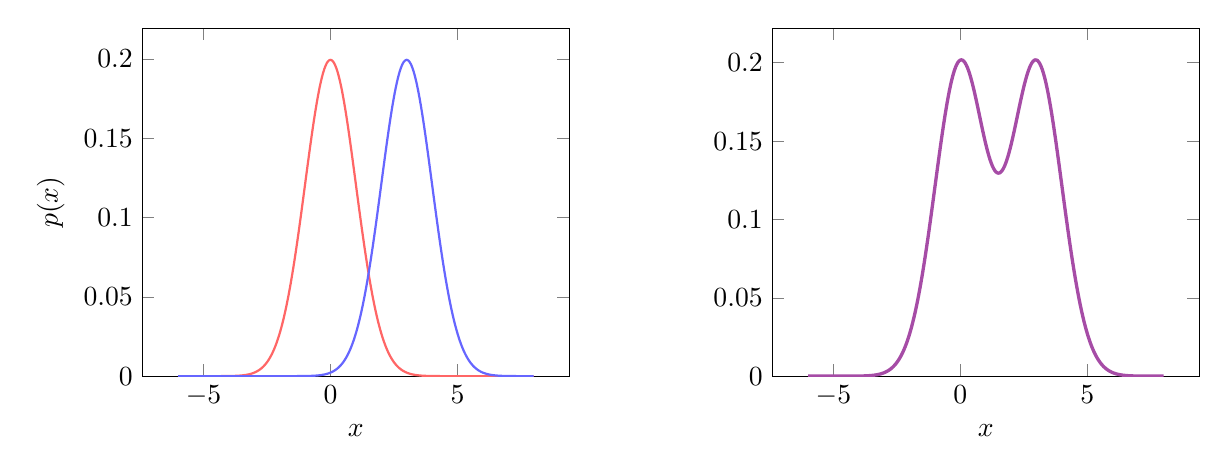
\begin{tikzpicture}

% ---------- Left plot: individual components ----------
\begin{axis}[
    at={(0,0)},
    anchor=south west,
    domain=-6:8,
    samples=300,
    width=7cm,
    height=6cm,
    xlabel={$x$},
    ylabel={$p(x)$},
    ymin=0,
    scaled y ticks=false,
    yticklabel style={
        /pgf/number format/fixed,
        /pgf/number format/precision=3
    }
]

% Soft red component
\addplot[
    thick,
    color=red!60
]
{0.5*(1/sqrt(2*pi)) * exp(-(x-0)^2/2)};

% Soft blue component
\addplot[
    thick,
    color=blue!60
]
{0.5*(1/sqrt(2*pi)) * exp(-(x-3)^2/2)};

\end{axis}

% ---------- Right plot: mixture ----------
\begin{axis}[
    at={(8cm,0)},
    anchor=south west,
    domain=-6:8,
    samples=300,
    width=7cm,
    height=6cm,
    xlabel={$x$},
    ymin=0,
    scaled y ticks=false,
    yticklabel style={
        /pgf/number format/fixed,
        /pgf/number format/precision=3
    }
]

% Soft purple mixture
\addplot[
    very thick,
    color=violet!70
]
{0.5*(1/sqrt(2*pi)) * exp(-(x-0)^2/2)
 +0.5*(1/sqrt(2*pi)) * exp(-(x-3)^2/2)};

\end{axis}

\end{tikzpicture}


This allows GMMs to model complex distributions that cannot be captured by a single normal distribution. Note that if we simply added two Gaussian densities together, the total area under the curve would be 2, so the result would no longer be a valid probability density. In a Gaussian mixture model, we instead take weighted proportions of each component, with weights that sum to 1. This ensures that the overall mixture still integrates to 1 and remains a proper probability distribution.

\bigskip

\subsection{Parameter Estimation via the EM Algorithm}

\medskip

The parameters of a Gaussian Mixture Model are typically estimated using the \emph{Expectation–Maximization} (EM) algorithm. Because the component labels are unobserved (we do not know which Gaussian generated each data point), direct maximization of the likelihood is not straightforward. The EM procedure addresses this difficulty by alternating between estimating cluster memberships and updating the model parameters.

\medskip

The algorithm proceeds as follows:

\begin{enumerate}[itemsep=0.8em]
    \item \textbf{Initialization.}
    Choose initial values for the parameters
    \[
    \{\mu_k, \Sigma_k, \pi_k\}_{k=1}^K.
    \]
    These may be selected randomly or obtained from a simpler
    clustering method such as $K$-means. Since the likelihood is not
    globally concave, initialization can influence the final solution.

    \item \textbf{Expectation Step (E-step).}
    Using the current parameter values, compute the probability that
    each observation belongs to each component. For each data point
    $x_i$, this produces a set of posterior probabilities that sum to 1.
    These values quantify soft cluster membership.

    \item \textbf{Maximization Step (M-step).}
    Update the parameters $\mu_k$, $\Sigma_k$, and $\pi_k$ so as to
    maximize the likelihood of the observed data, given the current
    membership probabilities. In effect, the parameters are re-estimated
    using weighted versions of the data.

    \item \textbf{Convergence.}
    Repeat the E-step and M-step until the parameter estimates stabilize
    or the increase in log-likelihood becomes negligible.
\end{enumerate}

Thus, EM alternates between estimating latent structure (cluster
membership probabilities) and optimizing the parameters conditional
on that structure. The procedure produces a sequence of parameter
estimates with non-decreasing likelihood, converging to a local maximum.

\bigskip

\subsection{Applications \& Limitations}

\medskip

GMM has applications in areas with complex data, such as speech recognition, finance, and image processing. The limitations of GMM include:

\begin{enumerate}[itemsep=0.5em]
    \item \textbf{Gaussian component assumption.} 
    GMM assumes the data are generated from a finite mixture of Gaussian components, 
    which implies ellipsoidal cluster shapes. If the true structure is strongly 
    non-Gaussian or heavy-tailed, the model may fit poorly or require many components.

    \item \textbf{Computational cost.} 
    The EM algorithm can be computationally expensive, especially in 
    high-dimensional settings where estimating full covariance matrices 
    scales poorly with dimension.

    \item \textbf{Sensitivity to initialization.} 
    The EM algorithm converges to a local maximum of the likelihood. 
    As a result, different initializations can lead to different solutions.

    \item \textbf{Choice of number of components.} 
    The number of mixture components $K$ is not determined automatically 
    and must be selected using model selection criteria such as BIC or AIC.
\end{enumerate}

